% 编译使用xelatex编译一次

\documentclass[12pt, a4paper, oneside]{ctexart}
\usepackage{subcaption,listings,amsmath, amsthm, amssymb, bm, booktabs, color, framed,float, graphicx, hyperref, mathrsfs,minipage-marginpar}

\title{\textbf{数据库系统作业五}}
\author{2021113140符世博}
\date{}
\linespread{1.5}
\definecolor{shadecolor}{RGB}{241, 241, 255}
\newcounter{problemname}
\newenvironment{problem}{\begin{shaded}\stepcounter{problemname}\par\noindent\textbf{题目\arabic{problemname}. }}{\end{shaded}\par}
\newenvironment{solution}{\par\noindent\textbf{解答. }}{\par}
\newenvironment{note}{\par\noindent\textbf{题目\arabic{problemname}的注记. }}{\par}

\begin{document}
\maketitle

% 1
\begin{problem}

考虑下面表中给出了 DBMS 对某四个事务操作五个数据项的调度按时间分布的表,其中
$R(X)$和$W(X)$分别代表了对数据项$X$的“读”和“写”。$T_i$表示事务$i$,$t_n$表示第$n$个时刻,请阅读
下表,并回答以下几个问题:

\begin{table}[H]
    \begin{center}
        \resizebox{\textwidth}{!}{
            \begin{tabular}{c|c|c|c|c|c|c|c|c|c|c|c}
                $time$ & $t_1$  & $t_2$  & $t_3$  & $t_4$  & $t_5$  & $t_6 $ & $t_7$  & $t_8$  & $t_9$  & $t_{10}$ & $t_{11}$ \\
                \hline
                $T_1 $ & $R(A)$ &        &        & $R(C)$ &        &        & $R(B)$ &        & $W(C)$ &          &          \\
                \hline
                $T_2 $ &        &        &        &        &        & $R(C)$ &        &        &        & $W(D)$   & $W(E)$   \\
                \hline
                $T_3 $ &        & $R(E)$ &        &        & $W(A)$ &        &        &        &        &          &          \\
                \hline
                $T_4 $ &        &        & $W(B)$ &        &        &        &        & $R(D)$ &        &          &          \\
            \end{tabular}
        }
    \end{center}
\end{table}

(1)\quad 这是否是一个串行的调度?

(2)\quad 请仿照课上幻灯片中的画法,画出上表中所示事务的优先图(请在箭头上表明实务操作的数据项)

(3)\quad 根据画出的事务优先图,该调度是否是个冲突可串行的调度?

\end{problem}

\begin{solution}

\end{solution}

% 2
\begin{problem}
设$r_i(X)$与$w_i(X)$分别表示事物$T_i$读、写数据单元$X$,则一个并发调度可以抽象为读、写
串。基于上述表示,画出优先图,并判断下面两个并发调度是否是可串行化的,为什么?

调度$S_1$:

$r_2(A);r_1(B);w_2(A);r_2(B);r_3(A);w_1(B);w_3(B);w_2(B)$

调度$S_2$:

$r_2(A);r_1(B);w_2(A);r_3(A);w_1(B);w_3(A);r_2(B);w_2(B)$
\end{problem}

\begin{solution}

\end{solution}

% 3
\begin{problem}
假设我校淘乐果园水果店架设了一套数据库系统,同学在超市挑选好商品后,带商品到
结算处结算付款,结算处有多名收银员使用多台机器进行结算。收银员负责扫同学购买水果
的种类和数量,由系统后台结算程序计算出同学购买商品的总金额,修改商品表的水果库存
量,并将销售信息写入销售表。请根据上述描述,回答以下问题。

假设有两位同学同时购买同一种类的水果,结算事务修改该水果的库存量(记为数据项)
所产生的部分调度如下表所示:

\begin{table}[H]
    \begin{center}

        \begin{tabular}{|c|c|}
            \hline
            $T1$                  & $T2$                  \\
            \hline
            $a\leftarrow Read(X)$ &                       \\
            \hline
                                  & $a\leftarrow Read(X)$ \\
            \hline
            $a=a-1$               &                       \\
            \hline
            $Write(X,a)$          &                       \\
            \hline
                                  & $a=a-2$               \\
            \hline
                                  & $Write(X,a)$          \\
            \hline
        \end{tabular}

    \end{center}
\end{table}

(1)\quad 如果数据项$X$购买前的初值为$114514$,则上述调度执行完成后,$X$的值是多少?这属于哪一类不一致性?

(2)\quad 引入独占锁指令$lock()$和解锁指令$Unlock()$,对"问题1"中存在并发调度进行重写,要求满足两段锁协议,且事务T1、T2首条指令的相对请求时间与"问题1"中的相同。


\end{problem}

\begin{solution}

\end{solution}

% 4
\begin{problem}
已知某数据库采用即时更新方法(undo-redo方法)记录WAL日志。设故障发生时WAL日志文件如下:
\begin{table}[H]
    \begin{center}
        \begin{tabular}{|l|}
            \hline
            $<T1,begin>$               \\
            $<T1,A,114,114514>$        \\
            $<T2,begin>$               \\
            $<T2,B,"hit","hitcs">$     \\
            $<T1,commit>$              \\
            $<T3,begin>$               \\
            $<T3,B,"hitcs","hitcsdb">$ \\
            $<T2,A,114514,1919810>$    \\
            \hline
        \end{tabular}
    \end{center}
\end{table}
当系统重启后,DBMS基于该WAL日志文件进行故障恢复。回答下列问题:

(1)\quad 该数据库系统的的日志恢复策略为Undo/Redo型,那么其对应的缓冲区处理策略是什
么(Steal?No Steal + Force?No Force)?该策略的每一项的具体内容都有什么?

(2)\quad 当DBMS进行故障恢复时,需要对那些事务进行undo?对那些事务进行redo?给出
具体理由

(3)\quad 当故障恢复完成时,对象A和B的值分别是什么?描述故障恢复的具体过程。
\end{problem}

\begin{solution}

\end{solution}

% 5
\begin{problem}
当前有一个支持故障恢复技术的DBMS,其采用了STEAL和NO-FORCE缓冲区策略,
假设每当DBMS执行检查点时会将数据缓冲区里面所有的脏数据块写入相应的数据文件,
保证数据库的一致性。

以下是数据库发生故障后的一份WAL日志,请阅读该日志并回答以下几个问题,

\begin{table}[H]
    \begin{center}
        \begin{tabular}{|rl|}
            \hline
            $\textbf{LSN}$ & $\textbf{WAL Record}$   \\
            $1$            & $<T1,BEGIN>$            \\
            $2$            & $<T1,X,1,2>$            \\
            $3$            & $<T2,BEGIN>$            \\
            $4$            & $<T2,Y,1,2>$            \\
            $5$            & $<T1,COMMIT>$           \\
            $6$            & $<T2,Y,2,3>$            \\
            $7$            & $<T3,BEGIN>$            \\
            $8$            & $<T3,Z,1,2>$            \\
            $9$            & $<T2,X,2,3>$            \\
            $10$           & $<\textbf{CHECKPOINT}>$ \\
            $11$           & $<T2,Y,3,4>$            \\
            $12$           & $<T3,Z,2,3>$            \\
            $13$           & $<T3,COMMIT>$           \\
            $14$           & $<T2,Z,3,4>$            \\
            \hline
        \end{tabular}
    \end{center}
\end{table}

其中,$<Ti,X,A,B>$分别代表事务$Ti$,数据项$X$,更新前数据项的值$A$,更新后数据项的值$B$

(1)\quad 请问DBMS需要进行恢复数据的时候,数据库的磁盘文件上数据项$X$、$Y$、$Z$的值分别是
多少?

(2)\quad 在对该WAL日志进行故障恢复的时候,事务$T1$、$T2$、$T3$都应如何处理?请详述该过程与
原因

(3)\quad 假设恢复作业完成后,DBMS会将所有的数据写入磁盘,DBMS从WAL恢复数据库
状态后数据库磁盘中数据项$X$、$Y$、$Z$的值分别是多少?
\end{problem}

\begin{solution}

\end{solution}

% 6
\begin{problem}
使用检查点的数据库恢复系统将根据事务的状态和检查点的关系采取相对应的恢复策
略,现在有事务$T_1-T_5$其执行过程如下图所示(线段左端和右端分别表示事务开始与提
交),其执行过程中数据库系统发生如图所示的故障,请回答下列问题

\begin{figure}[H]
    \centering
    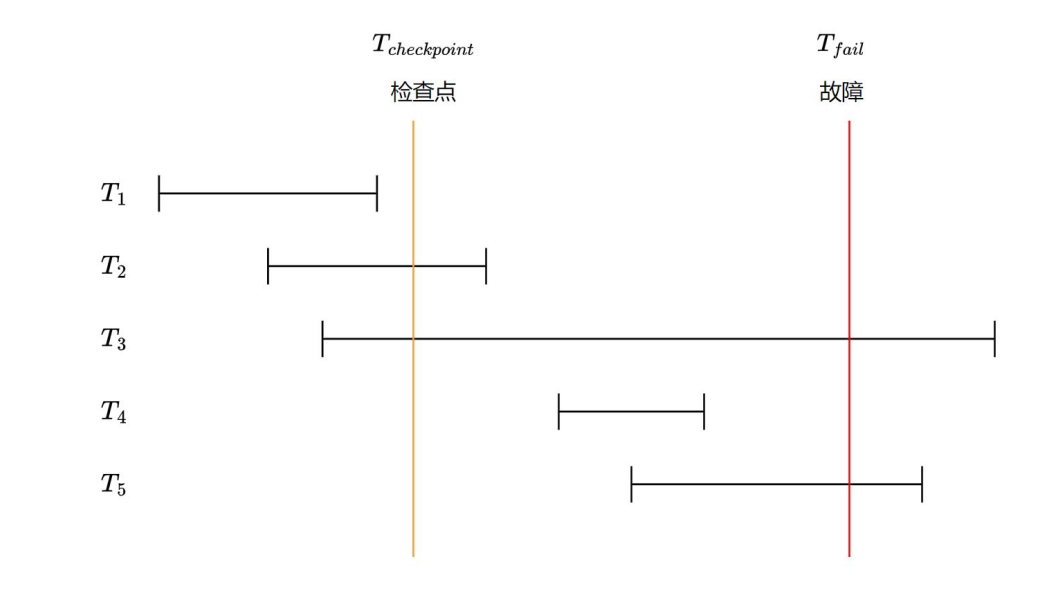
\includegraphics[width=0.9\textwidth]{figures/1.png}
\end{figure}

(1)\quad 请问在故障恢复时事务$T_1-T_5$那些需要撤销,那些需要重做,那些不需要操作?

(2)\quad 事务$T_6-T_8$的日志文件如下图所示,$<T_i,begin>$表示事务$T_i$开始执行,$<T_i,commit>$表示
事务提交,$<T_i,D,V_1,V_2>$表示事务$T_i$将数据项$D$的值由$V_1$修改为$V_2$,$<crash>$表
示数据库发生故障

\begin{table}[H]
    \begin{center}
        \begin{tabular}{|l|}
            \hline
            $<T_6,begin>$   \\
            $<T_6,X,100,1>$ \\
            $<T_7,begin>$   \\
            $<T_7,X,1,3>$   \\
            $<T_8,begin>$   \\
            $<T_7,Y,50,6>$  \\
            $<T_8,Y,6,8>$   \\
            $<T_8,Z,10,9>$  \\
            $<checkpoint>$  \\
            $<T_6,commit>$  \\
            $<T_8,Z,9,10>$  \\
            $<crash>$       \\
            \hline
        \end{tabular}
    \end{center}
\end{table}

数据库系统发生故障时,请给出恢复子系统时需要undo的事务列表和需要redo的事务列表

(3)\quad 请简述$T_6-T_8$在系统故障后基于检查点的故障恢复过程

\end{problem}

\begin{solution}

\end{solution}


\end{document}